% Options for packages loaded elsewhere
\PassOptionsToPackage{unicode}{hyperref}
\PassOptionsToPackage{hyphens}{url}
%
\documentclass[
]{article}
\usepackage{amsmath,amssymb}
\usepackage{iftex}
\ifPDFTeX
  \usepackage[T1]{fontenc}
  \usepackage[utf8]{inputenc}
  \usepackage{textcomp} % provide euro and other symbols
\else % if luatex or xetex
  \usepackage{unicode-math} % this also loads fontspec
  \defaultfontfeatures{Scale=MatchLowercase}
  \defaultfontfeatures[\rmfamily]{Ligatures=TeX,Scale=1}
\fi
\usepackage{lmodern}
\ifPDFTeX\else
  % xetex/luatex font selection
\fi
% Use upquote if available, for straight quotes in verbatim environments
\IfFileExists{upquote.sty}{\usepackage{upquote}}{}
\IfFileExists{microtype.sty}{% use microtype if available
  \usepackage[]{microtype}
  \UseMicrotypeSet[protrusion]{basicmath} % disable protrusion for tt fonts
}{}
\makeatletter
\@ifundefined{KOMAClassName}{% if non-KOMA class
  \IfFileExists{parskip.sty}{%
    \usepackage{parskip}
  }{% else
    \setlength{\parindent}{0pt}
    \setlength{\parskip}{6pt plus 2pt minus 1pt}}
}{% if KOMA class
  \KOMAoptions{parskip=half}}
\makeatother
\usepackage{xcolor}
\usepackage[left=2cm,right=2cm,top=1.5cm,bottom=1.5cm]{geometry}
\usepackage{color}
\usepackage{fancyvrb}
\newcommand{\VerbBar}{|}
\newcommand{\VERB}{\Verb[commandchars=\\\{\}]}
\DefineVerbatimEnvironment{Highlighting}{Verbatim}{commandchars=\\\{\}}
% Add ',fontsize=\small' for more characters per line
\usepackage{framed}
\definecolor{shadecolor}{RGB}{248,248,248}
\newenvironment{Shaded}{\begin{snugshade}}{\end{snugshade}}
\newcommand{\AlertTok}[1]{\textcolor[rgb]{0.94,0.16,0.16}{#1}}
\newcommand{\AnnotationTok}[1]{\textcolor[rgb]{0.56,0.35,0.01}{\textbf{\textit{#1}}}}
\newcommand{\AttributeTok}[1]{\textcolor[rgb]{0.13,0.29,0.53}{#1}}
\newcommand{\BaseNTok}[1]{\textcolor[rgb]{0.00,0.00,0.81}{#1}}
\newcommand{\BuiltInTok}[1]{#1}
\newcommand{\CharTok}[1]{\textcolor[rgb]{0.31,0.60,0.02}{#1}}
\newcommand{\CommentTok}[1]{\textcolor[rgb]{0.56,0.35,0.01}{\textit{#1}}}
\newcommand{\CommentVarTok}[1]{\textcolor[rgb]{0.56,0.35,0.01}{\textbf{\textit{#1}}}}
\newcommand{\ConstantTok}[1]{\textcolor[rgb]{0.56,0.35,0.01}{#1}}
\newcommand{\ControlFlowTok}[1]{\textcolor[rgb]{0.13,0.29,0.53}{\textbf{#1}}}
\newcommand{\DataTypeTok}[1]{\textcolor[rgb]{0.13,0.29,0.53}{#1}}
\newcommand{\DecValTok}[1]{\textcolor[rgb]{0.00,0.00,0.81}{#1}}
\newcommand{\DocumentationTok}[1]{\textcolor[rgb]{0.56,0.35,0.01}{\textbf{\textit{#1}}}}
\newcommand{\ErrorTok}[1]{\textcolor[rgb]{0.64,0.00,0.00}{\textbf{#1}}}
\newcommand{\ExtensionTok}[1]{#1}
\newcommand{\FloatTok}[1]{\textcolor[rgb]{0.00,0.00,0.81}{#1}}
\newcommand{\FunctionTok}[1]{\textcolor[rgb]{0.13,0.29,0.53}{\textbf{#1}}}
\newcommand{\ImportTok}[1]{#1}
\newcommand{\InformationTok}[1]{\textcolor[rgb]{0.56,0.35,0.01}{\textbf{\textit{#1}}}}
\newcommand{\KeywordTok}[1]{\textcolor[rgb]{0.13,0.29,0.53}{\textbf{#1}}}
\newcommand{\NormalTok}[1]{#1}
\newcommand{\OperatorTok}[1]{\textcolor[rgb]{0.81,0.36,0.00}{\textbf{#1}}}
\newcommand{\OtherTok}[1]{\textcolor[rgb]{0.56,0.35,0.01}{#1}}
\newcommand{\PreprocessorTok}[1]{\textcolor[rgb]{0.56,0.35,0.01}{\textit{#1}}}
\newcommand{\RegionMarkerTok}[1]{#1}
\newcommand{\SpecialCharTok}[1]{\textcolor[rgb]{0.81,0.36,0.00}{\textbf{#1}}}
\newcommand{\SpecialStringTok}[1]{\textcolor[rgb]{0.31,0.60,0.02}{#1}}
\newcommand{\StringTok}[1]{\textcolor[rgb]{0.31,0.60,0.02}{#1}}
\newcommand{\VariableTok}[1]{\textcolor[rgb]{0.00,0.00,0.00}{#1}}
\newcommand{\VerbatimStringTok}[1]{\textcolor[rgb]{0.31,0.60,0.02}{#1}}
\newcommand{\WarningTok}[1]{\textcolor[rgb]{0.56,0.35,0.01}{\textbf{\textit{#1}}}}
\usepackage{graphicx}
\makeatletter
\def\maxwidth{\ifdim\Gin@nat@width>\linewidth\linewidth\else\Gin@nat@width\fi}
\def\maxheight{\ifdim\Gin@nat@height>\textheight\textheight\else\Gin@nat@height\fi}
\makeatother
% Scale images if necessary, so that they will not overflow the page
% margins by default, and it is still possible to overwrite the defaults
% using explicit options in \includegraphics[width, height, ...]{}
\setkeys{Gin}{width=\maxwidth,height=\maxheight,keepaspectratio}
% Set default figure placement to htbp
\makeatletter
\def\fps@figure{htbp}
\makeatother
\setlength{\emergencystretch}{3em} % prevent overfull lines
\providecommand{\tightlist}{%
  \setlength{\itemsep}{0pt}\setlength{\parskip}{0pt}}
\setcounter{secnumdepth}{-\maxdimen} % remove section numbering
\ifLuaTeX
  \usepackage{selnolig}  % disable illegal ligatures
\fi
\usepackage{bookmark}
\IfFileExists{xurl.sty}{\usepackage{xurl}}{} % add URL line breaks if available
\urlstyle{same}
\hypersetup{
  hidelinks,
  pdfcreator={LaTeX via pandoc}}

\author{}
\date{\vspace{-2.5em}}

\begin{document}

\newcommand{\hoofding}[5]{
\begin{flushleft}
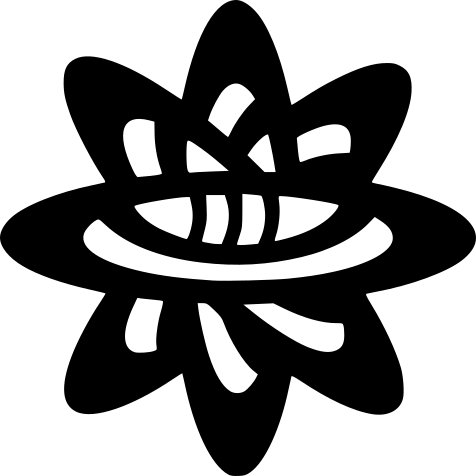
\includegraphics[height=2cm]{ecfmlogo.png}
\end{flushleft}
\vspace{-2.5cm}
\hspace{2.5cm} 
\parbox{12cm}{ #1\\#2\\#3\\#4\\#5} 

{\parindent=0pt \hrulefill} 
\vspace{1mm}}

\newcommand{\encabezadorep}[9]{
\begin{flushleft}
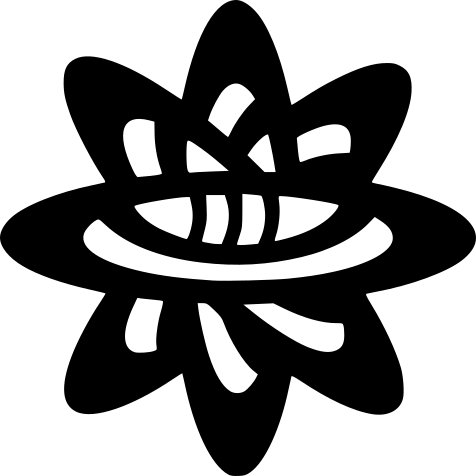
\includegraphics[height=2cm]{ecfmlogo.png}
\end{flushleft}
\vspace{-2.7cm}
\hspace{2.5cm} 
\parbox{12cm}{ #1\\#2\\#3\\#4 \hspace{0.6cm} #5\\#6 \hspace{0.6cm} #7\\#8 \hspace{0.6cm} #9} 

{\parindent=0pt \hrulefill} 
\vspace{1mm}}

\begin{flushleft}
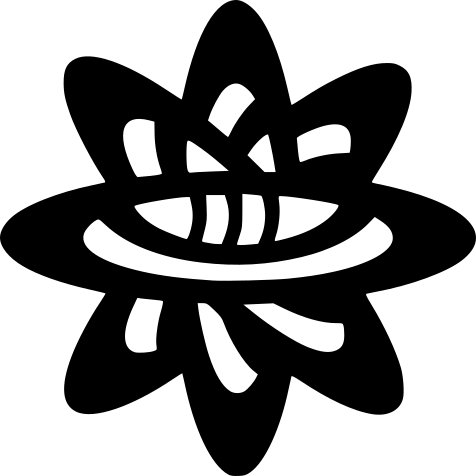
\includegraphics[height=2cm]{ecfmlogo.png}
\end{flushleft}
\vspace{-2.5cm}
\hspace{2.5cm} 
\parbox{12cm}{ ESCUELA DE CIENCIAS FISÍCAS Y MATEMÁTICAS\\LABORATORIO DE REDUCCIÓN DE DATOS\\ING. MAYNOR BALLINA\\LABORATORIO 2\\FECHA DE ENTREGA: 06/05/2022} 

{\parindent=0pt \hrulefill} 
\vspace{1mm}

\vspace{-1em}

\subsection{\texorpdfstring{\textbf{Instrucciones para el experimento
}}{Instrucciones para el experimento }}\label{instrucciones-para-el-experimento}

\subsubsection{\texorpdfstring{\textbf{Definir el tamaño de la muestra
}}{Definir el tamaño de la muestra }}\label{definir-el-tamauxf1o-de-la-muestra}

\begin{enumerate}
\def\labelenumi{\arabic{enumi}.}
\tightlist
\item
  Defina el tamaño de las muestras a utilizar dependiendo del intervalo
  de confianza a utilizar y el error requerido.
\end{enumerate}

\begin{figure}
  \centering
  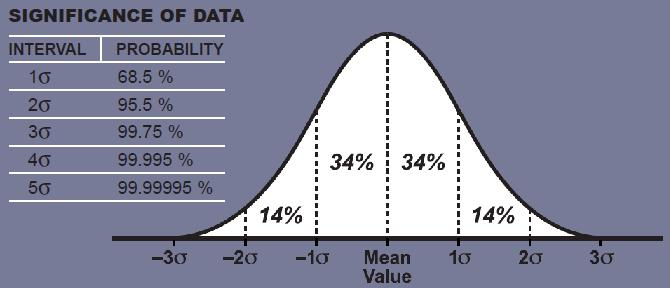
\includegraphics[height=3cm]{intervalo_confianza.jpg}
\end{figure}

\begin{table}[ht]
\centering
\caption{Calculo del tamaño de la muestra}
\begin{tabular}{ccc}
Error estadístico & Intervalo de confianza & n \\  \hline
$20\%$ & $1 \sigma$ & \\
$20\%$ & $2 \sigma$ & \\
$20\%$ & $3 \sigma$ & \\
$20\%$ & $4 \sigma$ & \\
$20\%$ & $5 \sigma$ & \\
$5\%$ & $1 \sigma$ & \\
$5\%$ & $2 \sigma$ & \\
$5\%$ & $3 \sigma$ & \\
$5\%$ & $4 \sigma$ & \\
$5\%$ & $5 \sigma$ & \\
$1\%$ & $2 \sigma$ & \\
$0.1\%$ & $2 \sigma$ & \\
$0.01\%$ & $2 \sigma$ & \\
$0.001\%$ & $2 \sigma$ & \\
$0.0001\%$ & $2 \sigma$ & \\
\hline
\end{tabular}
\end{table}

\begin{enumerate}
\def\labelenumi{\arabic{enumi}.}
\setcounter{enumi}{1}
\item
  Realice gráficos que le ayuden a determinar que elemento (IC, Error)
  hace que el tamaño de la muestra aumente mas.
\item
  Desde su punto de vista describa que es mas importante, tener un error
  estadístico bastante pequeño o una significativa muy pequeña.
\item
  El tamaño de muestra para su experimento es el obtenido para un
  intervalo de confianza de \(5 \sigma\) y un error estadístico del
  \(5\%\)
\end{enumerate}

TODAS ESTOS PUNTOS SE EXPLICARÁN EN LAS CONCLUSIONES.

\subsubsection{\texorpdfstring{\textbf{Procedimiento pendulo simple
}}{Procedimiento pendulo simple }}\label{procedimiento-pendulo-simple}

\begin{enumerate}
\def\labelenumi{\arabic{enumi}.}
\tightlist
\item
  Armar un sistema de péndulo debe crear un péndulo que mida un metro y
  una masa grande (se recomienda un péndulo hecho con un hilo, para que
  la masa del hilo sea despreciable, con una longitud de por lo menos
  metro y medio).
\item
  Medir la longitud del péndulo, recuerde este es desde el punto de
  sujeción hasta el centro de masa del objeto.
\item
  Coloque el péndulo a un ángulo no mayor de \(5^o\), suelte, inicie a
  medir, con el cronometro, el periodo de oscilación de 10 oscilaciones
  consecutivas. (ojo el periodo es corto, por lo cual necesita un
  cronometro que mida centisegundo.)
\item
  El valor del periodo promedio de las 10 oscilaciones esta dado por:
  \[T=\frac{t}{n}\]
\item
  Realice el procedimiento anterior 100 veces para tener una muestra de
  1000 oscilaciones.
\item
  Realice un histograma de frecuencias de los datos obtenidos.
\item
  Tomando en cuenta los resultados de la tabla realice el calculo del
  periodo promedio y su desviación estándar para cada intervalo de
  confianza, recuerde tomar en cuenta el tamaño de la muestra necesaria.
  Calcule el valor de la gravedad para cada intervalo de confianza.
  (recuerde que debe de utilizar propagación de error) Llene la
  siguiente tabla.
\end{enumerate}

\begin{table}[ht]
\centering
\caption{Calculo del la gravedad}
\begin{tabular}{ccccccc}
Error estadístico & IC & n & T & $\Delta$T & g & $\Delta$g \\  \hline
$20\%$ & $1 \sigma$ & n1 & media1 & $\pm 0.01$ & g1 &\\
$20\%$ & $2 \sigma$ & n2 & media2 & $\pm 0.03$ & g2 &\\
$20\%$ & $3 \sigma$ & n3 & media3 & $\pm 0.06$ & g3 &\\
$20\%$ & $4 \sigma$ & n4 & media4 & $\pm 0.010$ & g4 &\\
$20\%$ & $5 \sigma$ & n5 & media5 & $\pm 0.016$ & g5 &\\
$5\%$ & $1 \sigma$ & n6 & media6 & $\pm 0.01$& g6 &\\
$5\%$ & $2 \sigma$ & n7 & media7 & $\pm 0.40$& g7 &\\
$5\%$ & $3 \sigma$ & n8 & media8 & $\pm 0.90$& g8 &\\
\hline
\end{tabular}
\end{table}

EN LOS RESULTADOS SE ENCUENTRAN DETALLADAMENTE LOS DATOS SOLICITADOS EN
LA TABLA.

\begin{enumerate}
\def\labelenumi{\arabic{enumi}.}
\setcounter{enumi}{7}
\tightlist
\item
  Con las muestras obtenidas, utilice bootstraping para generar las
  muestras para poder completar la siguiente tabla
\end{enumerate}

\begin{table}[ht]
\centering
\caption{Calculo del la gravedad con bootstraping}
\begin{tabular}{ccccccc}
Error estadístico & IC & n & T & $\Delta$T & g & $\Delta$g \\  \hline
$5\%$ & $4 \sigma$ & \\
$5\%$ & $5 \sigma$ & \\
$1\%$ & $2 \sigma$ & \\
\hline
\end{tabular}
\end{table}

\begin{enumerate}
\def\labelenumi{\arabic{enumi}.}
\setcounter{enumi}{8}
\tightlist
\item
  Realice una gráfica para ver el comportamiento de los valores de
  gravedad obtenidos.
\item
  Realice una gráfica para ver el comportamiento de los residuos tomando
  en cuenta que el valor real de la gravedad es de 9,80665 \(m/s^2\)
\end{enumerate}

\newpage

\begin{flushleft}
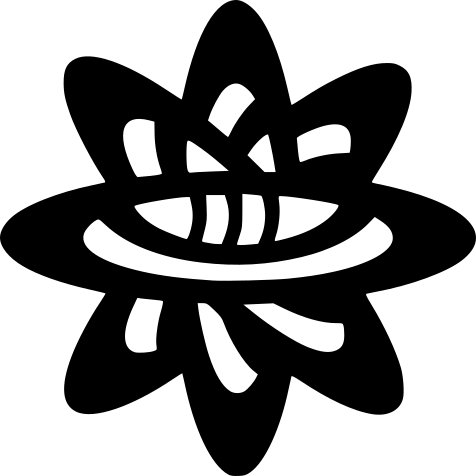
\includegraphics[height=2cm]{ecfmlogo.png}
\end{flushleft}
\vspace{-2.7cm}
\hspace{2.5cm} 
\parbox{12cm}{ ESCUELA DE CIENCIAS FISÍCAS Y MATEMÁTICAS\\LABORATORIO DE REDUCCIÓN DE DATOS\\LABORATORIO 2: INTERVALOS DE CONFIANZA Y ERROR\\NOMBRE: Gerson Figueroa \hspace{0.6cm} CARNET: 202005839 \\NOMBRE:  \hspace{0.6cm} CARNET:\\ \hspace{0.6cm} } 

{\parindent=0pt \hrulefill} 
\vspace{1mm}

\subsection{\texorpdfstring{\textbf{Resumen }}{Resumen }}\label{resumen}

El siguiente experimento aborda el calculo de la gravedad terrestre por
medio de un pendulo simple y el despeje de una ecuación (la cual está en
el anexo), la cual relaciona la gravedad con los datos empericos que se
pueden medir en el experimento. Con estos datos se busca a grandes
rasgos calcular los intervalos de confianza y error para los diferentes
valores de sigma. Además se analizan los datos estadisticamente para ver
el comportamiento de los mismos.

\subsection{\texorpdfstring{\textbf{Objetivos
}}{Objetivos }}\label{objetivos}

\begin{enumerate}
\def\labelenumi{\arabic{enumi}.}
\tightlist
\item
  Calcular el valor de la gravedad terrestre.
\item
  Armar un sistema de pendulo lo más exacto posible para tomar buenos
  datos.
\item
  Calcular los intervalos de confianza
\item
  Graficar el comportamiento de los datos. 5.Describir si es más
  importante tener un error estadístico bastante pequeño o una
  significativa muy pequeña.
\end{enumerate}

\subsection{\texorpdfstring{\textbf{Marco Teórico
}}{Marco Teórico }}\label{marco-teuxf3rico}

\begin{enumerate}
\def\labelenumi{\arabic{enumi}.}
\tightlist
\item
  Un intervalo de confianza es un rango de valores, derivado de los
  estadísticos de la muestra, que posiblemente incluya el valor de un
  parámetro de población desconocido. Debido a su naturaleza aleatoria,
  es poco probable que dos muestras de una población en particular
  produzcan intervalos de confianza idénticos. Sin embargo, si usted
  repitiera muchas veces su muestra, un determinado porcentaje de los
  intervalos de confianza resultantes incluiría el parámetro de
  población desconocido. Mientras mayor sea el margen de error, más
  ancho será el intervalo y menos seguro podrá estar usted del valor de
  la estimación de punto. 2.La diferencia entre un estadístico de
  muestra y un valor hipotético es estadísticamente significativa si una
  prueba de hipótesis indica que es muy poco probable que la misma haya
  ocurrido en virtud de las probabilidades. Para evaluar la
  significancia estadística, examine el valor p de la prueba. Si el
  valor p está por debajo de un nivel de significancia (α) especificado
  (generalmente 0.10, 0.05 o 0.01), usted puede decir que la diferencia
  es estadísticamente significativa y rechazar la hipótesis nula de la
  prueba.La significancia estadística por sí sola no implica que los
  resultados tengan una consecuencia práctica. Si utiliza una prueba con
  una potencia muy alta, podría concluir que una pequeña diferencia con
  respecto al valor hipotético es estadísticamente significativa. Sin
  embargo, esa pequeña diferencia podría ser insignificante para su
  situación. Debe usar su conocimiento especializado para determinar si
  la diferencia es significativa desde el punto de vista práctico.
\item
  La propagación de errores es un procedimiento por medio del cual,
  asignamos un error a los resultados obtenidos, tras la aplicación de
  una fórmula física; es decir aquellas medidas que obtenemos
  indirectamente, teniendo como entrada datos experimentales, los cuales
  siempre tienen un nivel de incertidumbre conocido.
\end{enumerate}

Desde la física se trabajan tres tipos de errores:

Incertidumbre: son los ocasionados por la precisión del instrumento de
medida. Sistemáticos: Es el que se genera por defectos en las
mediciones, producto de errores en los instrumentos o en el encargado de
realizar la medida. Estadísticos: Este error hace referencia en que
tanto difiere una medida de un valor esperado. La asignación de errores
de hace dependiendo del origen de la medida obtenida, si es una medida
directa, indirecta o ponderada.

\subsection{\texorpdfstring{\textbf{Diseño Experimental
}}{Diseño Experimental }}\label{diseuxf1o-experimental}

Para hacer el sistema del pendulo se utilizó un hilo enrollado (para
mayor resistencia), de una longitud de un metro y la masa fue una pelota
esferica (para evitar en la mayor medida posible la resistencia del
aire) de una masa de 1kg. El pendulo se instaló en un cuarto sin
ventanas para evitar el aire y se alineo el extremo superior del pendulo
a un transpotador para así medir los 5 a los cuales debia salir el
pendulo. Los datos de tiempo fueron tomados con un cronometro de celular
que mide el tiempo con una precision de milisegundos.

\subsection{\texorpdfstring{\textbf{Resultados
}}{Resultados }}\label{resultados}

\begin{Shaded}
\begin{Highlighting}[]
\CommentTok{\#Datos de los periodos de las 10 oscilaciones:}
\NormalTok{T100}\OtherTok{=}\FunctionTok{c}\NormalTok{(}\FloatTok{20.75}\NormalTok{,}\FloatTok{20.08}\NormalTok{,}\FloatTok{19.70}\NormalTok{,}\FloatTok{19.35}\NormalTok{,}\FloatTok{19.65}\NormalTok{,}\FloatTok{20.45}\NormalTok{,}\FloatTok{20.33}\NormalTok{,}\FloatTok{19.84}\NormalTok{,}\FloatTok{19.58}\NormalTok{,}\FloatTok{19.46}\NormalTok{,}\FloatTok{19.98}\NormalTok{,}\FloatTok{20.05}\NormalTok{,}\FloatTok{20.35}\NormalTok{,}\FloatTok{19.22}\NormalTok{,}\FloatTok{19.71}\NormalTok{,}\FloatTok{19.99}\NormalTok{,}\FloatTok{21.01}\NormalTok{,}\FloatTok{20.56}\NormalTok{,}\FloatTok{20.41}\NormalTok{,}\FloatTok{20.80}\NormalTok{,}\FloatTok{21.09}\NormalTok{,}\FloatTok{20.98}\NormalTok{,}\FloatTok{19.45}\NormalTok{,}\FloatTok{20.05}\NormalTok{,}\FloatTok{20.79}\NormalTok{,}\FloatTok{21.01}\NormalTok{,}\FloatTok{20.23}\NormalTok{,}\FloatTok{20.55}\NormalTok{,}\FloatTok{20.44}\NormalTok{,}\FloatTok{20.96}\NormalTok{,}\FloatTok{20.74}\NormalTok{,}\FloatTok{20.54}\NormalTok{,}\FloatTok{19.27}\NormalTok{,}\FloatTok{19.56}\NormalTok{,}\FloatTok{20.14}\NormalTok{,}\FloatTok{20.75}\NormalTok{,}\FloatTok{20.46}\NormalTok{,}\FloatTok{19.42}\NormalTok{,}\FloatTok{20.89}\NormalTok{,}\FloatTok{20.89}\NormalTok{,}\FloatTok{19.63}\NormalTok{,}\FloatTok{19.71}\NormalTok{,}\FloatTok{19.36}\NormalTok{,}\FloatTok{20.11}\NormalTok{,}\FloatTok{20.85}\NormalTok{,}\FloatTok{20.65}\NormalTok{,}\FloatTok{20.65}\NormalTok{,}\FloatTok{19.87}\NormalTok{,}\FloatTok{20.55}\NormalTok{,}\FloatTok{20.82}\NormalTok{,}\FloatTok{21.03}\NormalTok{,}\FloatTok{20.00}\NormalTok{,}\FloatTok{20.74}\NormalTok{,}\FloatTok{19.03}\NormalTok{,}\FloatTok{18.50}\NormalTok{,}\FloatTok{20.90}\NormalTok{,}\FloatTok{20.01}\NormalTok{,}\FloatTok{19.45}\NormalTok{,}\FloatTok{19.54}\NormalTok{,}\FloatTok{19.03}\NormalTok{,}\FloatTok{20.22}\NormalTok{,}\FloatTok{20.64}\NormalTok{,}\FloatTok{20.44}\NormalTok{,}\FloatTok{19.52}\NormalTok{,}\FloatTok{20.10}\NormalTok{,}\FloatTok{19.43}\NormalTok{,}\FloatTok{20.87}\NormalTok{,}\FloatTok{20.13}\NormalTok{,}\FloatTok{20.15}\NormalTok{,}\FloatTok{20.85}\NormalTok{,}\FloatTok{20.41}\NormalTok{,}\FloatTok{20.11}\NormalTok{,}\FloatTok{20.23}\NormalTok{,}\FloatTok{20.21}\NormalTok{,}\FloatTok{20.33}\NormalTok{,}\FloatTok{19.01}\NormalTok{,}\FloatTok{19.05}\NormalTok{,}\FloatTok{19.32}\NormalTok{,}\FloatTok{19.41}\NormalTok{,}\FloatTok{20.55}\NormalTok{,}\FloatTok{20.66}\NormalTok{,}\FloatTok{20.21}\NormalTok{,}\FloatTok{20.63}\NormalTok{,}\FloatTok{19.21}\NormalTok{,}\FloatTok{19.32}\NormalTok{,}\FloatTok{19.31}\NormalTok{,}\FloatTok{19.25}\NormalTok{,}\FloatTok{19.17}\NormalTok{,}\FloatTok{19.19}\NormalTok{,}\FloatTok{20.11}\NormalTok{,}\FloatTok{19.50}\NormalTok{,}\FloatTok{19.15}\NormalTok{,}\FloatTok{20.00}\NormalTok{,}\FloatTok{20.16}\NormalTok{,}\FloatTok{19.19}\NormalTok{,}\FloatTok{20.36}\NormalTok{,}\FloatTok{20.41}\NormalTok{,}\FloatTok{19.20}\NormalTok{,}\FloatTok{19.25}\NormalTok{,}\FloatTok{19.02}\NormalTok{)}
\CommentTok{\#Notar que cada valor que está dentro del vector T100}
\CommentTok{\#es el periodo de 100 oscilaciones.}

\CommentTok{\#Hacemos el histograma de los datos obtenidos:}
\FunctionTok{hist}\NormalTok{(T100, }\AttributeTok{main =} \StringTok{"Histograma de oscilaciones"}\NormalTok{, }\AttributeTok{ylab =} \StringTok{"veces que se repite el dato"}\NormalTok{, }\AttributeTok{xlab =} \StringTok{"Tiempo de las 10 oscilaciones"}\NormalTok{)}
\end{Highlighting}
\end{Shaded}

\begin{center}\includegraphics[width=0.6\linewidth,height=0.6\textheight]{Laboratorio2_files/figure-latex/unnamed-chunk-1-1} \end{center}

\begin{Shaded}
\begin{Highlighting}[]
\NormalTok{media}\OtherTok{=}\FunctionTok{mean}\NormalTok{(T100)}
\FunctionTok{sd}\NormalTok{(T100)}
\end{Highlighting}
\end{Shaded}

\begin{verbatim}
## [1] 0.631648
\end{verbatim}

\begin{Shaded}
\begin{Highlighting}[]
\CommentTok{\#Calculo de la gravedad:}
\NormalTok{longitud}\OtherTok{=}\DecValTok{1}
\NormalTok{g}\OtherTok{=}\DecValTok{4}\SpecialCharTok{*}\NormalTok{pi}\SpecialCharTok{\^{}}\DecValTok{2}\SpecialCharTok{*}\NormalTok{longitud}\SpecialCharTok{/}\NormalTok{(media}\SpecialCharTok{/}\DecValTok{10}\NormalTok{)}\SpecialCharTok{\^{}}\DecValTok{2}\NormalTok{;g}
\end{Highlighting}
\end{Shaded}

\begin{verbatim}
## [1] 9.82838
\end{verbatim}

\begin{Shaded}
\begin{Highlighting}[]
\CommentTok{\#Calculo de la gravedad para cada intervalo de }
\CommentTok{\#confianza}
\CommentTok{\#Para un error del 20\% y un indice de confianza de}
\CommentTok{\#un sigma}
\NormalTok{sigma }\OtherTok{\textless{}{-}} \FunctionTok{c}\NormalTok{(}\FloatTok{68.5}\NormalTok{,}\FloatTok{95.5}\NormalTok{,}\FloatTok{99.75}\NormalTok{,}\FloatTok{99.995}\NormalTok{,}\FloatTok{99.99995}\NormalTok{)}
\NormalTok{error1}\OtherTok{=}\DecValTok{20}\SpecialCharTok{/}\DecValTok{100}
\NormalTok{alfa.medios1 }\OtherTok{\textless{}{-}}\NormalTok{ (}\DecValTok{100}\SpecialCharTok{{-}}\NormalTok{sigma[}\DecValTok{1}\NormalTok{])}\SpecialCharTok{/}\DecValTok{2}\SpecialCharTok{/}\DecValTok{100}\NormalTok{;alfa.medios1}
\end{Highlighting}
\end{Shaded}

\begin{verbatim}
## [1] 0.1575
\end{verbatim}

\begin{Shaded}
\begin{Highlighting}[]
\NormalTok{alfa.medios1}\SpecialCharTok{*}\DecValTok{2}
\end{Highlighting}
\end{Shaded}

\begin{verbatim}
## [1] 0.315
\end{verbatim}

\begin{Shaded}
\begin{Highlighting}[]
\NormalTok{z1 }\OtherTok{\textless{}{-}} \FunctionTok{qnorm}\NormalTok{(alfa.medios1, }\AttributeTok{lower.tail =}\NormalTok{ F);z1}
\end{Highlighting}
\end{Shaded}

\begin{verbatim}
## [1] 1.004786
\end{verbatim}

\begin{Shaded}
\begin{Highlighting}[]
\NormalTok{n1 }\OtherTok{\textless{}{-}}\NormalTok{ ((z1}\SpecialCharTok{*}\FloatTok{0.5}\NormalTok{)}\SpecialCharTok{/}\NormalTok{error1)}\SpecialCharTok{\^{}}\DecValTok{2}\NormalTok{;n1}
\end{Highlighting}
\end{Shaded}

\begin{verbatim}
## [1] 6.309966
\end{verbatim}

\begin{Shaded}
\begin{Highlighting}[]
\NormalTok{media1}\OtherTok{=}\NormalTok{(T100[}\DecValTok{1}\NormalTok{])}\SpecialCharTok{/}\DecValTok{1}
\NormalTok{g1}\OtherTok{=}\DecValTok{4}\SpecialCharTok{*}\NormalTok{pi}\SpecialCharTok{\^{}}\DecValTok{2}\SpecialCharTok{*}\NormalTok{longitud}\SpecialCharTok{/}\NormalTok{(media1}\SpecialCharTok{/}\DecValTok{10}\NormalTok{)}\SpecialCharTok{\^{}}\DecValTok{2}
\NormalTok{lim\_inferior1}\OtherTok{=}\NormalTok{g1}\SpecialCharTok{{-}}\NormalTok{(z1}\SpecialCharTok{*}\NormalTok{error1);lim\_inferior1}
\end{Highlighting}
\end{Shaded}

\begin{verbatim}
## [1] 8.968076
\end{verbatim}

\begin{Shaded}
\begin{Highlighting}[]
\NormalTok{lim\_superior1}\OtherTok{=}\NormalTok{g1}\SpecialCharTok{+}\NormalTok{(z1}\SpecialCharTok{*}\NormalTok{error1);lim\_superior1}
\end{Highlighting}
\end{Shaded}

\begin{verbatim}
## [1] 9.36999
\end{verbatim}

\begin{Shaded}
\begin{Highlighting}[]
\CommentTok{\#Para un indice de confianza de dos sigmas:}

\NormalTok{sigma }\OtherTok{\textless{}{-}} \FunctionTok{c}\NormalTok{(}\FloatTok{68.5}\NormalTok{,}\FloatTok{95.5}\NormalTok{,}\FloatTok{99.75}\NormalTok{,}\FloatTok{99.995}\NormalTok{,}\FloatTok{99.99995}\NormalTok{)}
\NormalTok{error2}\OtherTok{=}\DecValTok{20}\SpecialCharTok{/}\DecValTok{100}
\NormalTok{alfa.medios2 }\OtherTok{\textless{}{-}}\NormalTok{ (}\DecValTok{100}\SpecialCharTok{{-}}\NormalTok{sigma[}\DecValTok{2}\NormalTok{])}\SpecialCharTok{/}\DecValTok{2}\SpecialCharTok{/}\DecValTok{100}\NormalTok{;alfa.medios2}
\end{Highlighting}
\end{Shaded}

\begin{verbatim}
## [1] 0.0225
\end{verbatim}

\begin{Shaded}
\begin{Highlighting}[]
\NormalTok{alfa.medios2}\SpecialCharTok{*}\DecValTok{2}
\end{Highlighting}
\end{Shaded}

\begin{verbatim}
## [1] 0.045
\end{verbatim}

\begin{Shaded}
\begin{Highlighting}[]
\NormalTok{z2 }\OtherTok{\textless{}{-}} \FunctionTok{qnorm}\NormalTok{(alfa.medios2, }\AttributeTok{lower.tail =}\NormalTok{ F);z2}
\end{Highlighting}
\end{Shaded}

\begin{verbatim}
## [1] 2.004654
\end{verbatim}

\begin{Shaded}
\begin{Highlighting}[]
\NormalTok{n2 }\OtherTok{\textless{}{-}}\NormalTok{ ((z2}\SpecialCharTok{*}\FloatTok{0.5}\NormalTok{)}\SpecialCharTok{/}\NormalTok{error2)}\SpecialCharTok{\^{}}\DecValTok{2}\NormalTok{;n2}
\end{Highlighting}
\end{Shaded}

\begin{verbatim}
## [1] 25.1165
\end{verbatim}

\begin{Shaded}
\begin{Highlighting}[]
\NormalTok{media2}\OtherTok{=}\NormalTok{(T100[}\DecValTok{1}\NormalTok{]}\SpecialCharTok{+}\NormalTok{T100[}\DecValTok{2}\NormalTok{]}\SpecialCharTok{+}\NormalTok{T100[}\DecValTok{3}\NormalTok{])}\SpecialCharTok{/}\DecValTok{3}
\NormalTok{g2}\OtherTok{=}\DecValTok{4}\SpecialCharTok{*}\NormalTok{pi}\SpecialCharTok{\^{}}\DecValTok{2}\SpecialCharTok{*}\NormalTok{longitud}\SpecialCharTok{/}\NormalTok{(media2}\SpecialCharTok{/}\DecValTok{10}\NormalTok{)}\SpecialCharTok{\^{}}\DecValTok{2}
\NormalTok{lim\_inferior2}\OtherTok{=}\NormalTok{g2}\SpecialCharTok{{-}}\NormalTok{(z2}\SpecialCharTok{*}\NormalTok{error2);lim\_inferior2}
\end{Highlighting}
\end{Shaded}

\begin{verbatim}
## [1] 9.296594
\end{verbatim}

\begin{Shaded}
\begin{Highlighting}[]
\NormalTok{lim\_superior2}\OtherTok{=}\NormalTok{g2}\SpecialCharTok{+}\NormalTok{(z2}\SpecialCharTok{*}\NormalTok{error2);lim\_superior2}
\end{Highlighting}
\end{Shaded}

\begin{verbatim}
## [1] 10.09846
\end{verbatim}

\begin{Shaded}
\begin{Highlighting}[]
\CommentTok{\#Para un indice de confianza de tres sigmas:}

\NormalTok{sigma }\OtherTok{\textless{}{-}} \FunctionTok{c}\NormalTok{(}\FloatTok{68.5}\NormalTok{,}\FloatTok{95.5}\NormalTok{,}\FloatTok{99.75}\NormalTok{,}\FloatTok{99.995}\NormalTok{,}\FloatTok{99.99995}\NormalTok{)}
\NormalTok{error3}\OtherTok{=}\DecValTok{20}\SpecialCharTok{/}\DecValTok{100}
\NormalTok{alfa.medios3 }\OtherTok{\textless{}{-}}\NormalTok{ (}\DecValTok{100}\SpecialCharTok{{-}}\NormalTok{sigma[}\DecValTok{3}\NormalTok{])}\SpecialCharTok{/}\DecValTok{2}\SpecialCharTok{/}\DecValTok{100}\NormalTok{;alfa.medios3}
\end{Highlighting}
\end{Shaded}

\begin{verbatim}
## [1] 0.00125
\end{verbatim}

\begin{Shaded}
\begin{Highlighting}[]
\NormalTok{alfa.medios3}\SpecialCharTok{*}\DecValTok{2}
\end{Highlighting}
\end{Shaded}

\begin{verbatim}
## [1] 0.0025
\end{verbatim}

\begin{Shaded}
\begin{Highlighting}[]
\NormalTok{z3 }\OtherTok{\textless{}{-}} \FunctionTok{qnorm}\NormalTok{(alfa.medios3, }\AttributeTok{lower.tail =}\NormalTok{ F);z3}
\end{Highlighting}
\end{Shaded}

\begin{verbatim}
## [1] 3.023341
\end{verbatim}

\begin{Shaded}
\begin{Highlighting}[]
\NormalTok{n3 }\OtherTok{\textless{}{-}}\NormalTok{ ((z3}\SpecialCharTok{*}\FloatTok{0.5}\NormalTok{)}\SpecialCharTok{/}\NormalTok{error2)}\SpecialCharTok{\^{}}\DecValTok{2}\NormalTok{;n3}
\end{Highlighting}
\end{Shaded}

\begin{verbatim}
## [1] 57.12871
\end{verbatim}

\begin{Shaded}
\begin{Highlighting}[]
\NormalTok{media3}\OtherTok{=}\NormalTok{(T100[}\DecValTok{1}\NormalTok{]}\SpecialCharTok{+}\NormalTok{T100[}\DecValTok{2}\NormalTok{]}\SpecialCharTok{+}\NormalTok{T100[}\DecValTok{3}\NormalTok{]}\SpecialCharTok{+}\NormalTok{T100[}\DecValTok{4}\NormalTok{]}\SpecialCharTok{+}\NormalTok{T100[}\DecValTok{5}\NormalTok{]}\SpecialCharTok{+}\NormalTok{T100[}\DecValTok{6}\NormalTok{])}\SpecialCharTok{/}\DecValTok{6}
\NormalTok{g3}\OtherTok{=}\DecValTok{4}\SpecialCharTok{*}\NormalTok{pi}\SpecialCharTok{\^{}}\DecValTok{2}\SpecialCharTok{*}\NormalTok{longitud}\SpecialCharTok{/}\NormalTok{(media3}\SpecialCharTok{/}\DecValTok{10}\NormalTok{)}\SpecialCharTok{\^{}}\DecValTok{2}
\NormalTok{lim\_inferior3}\OtherTok{=}\NormalTok{g3}\SpecialCharTok{{-}}\NormalTok{(z3}\SpecialCharTok{*}\NormalTok{error3);lim\_inferior3}
\end{Highlighting}
\end{Shaded}

\begin{verbatim}
## [1] 9.268227
\end{verbatim}

\begin{Shaded}
\begin{Highlighting}[]
\NormalTok{lim\_superior3}\OtherTok{=}\NormalTok{g3}\SpecialCharTok{+}\NormalTok{(z3}\SpecialCharTok{*}\NormalTok{error3);lim\_superior3}
\end{Highlighting}
\end{Shaded}

\begin{verbatim}
## [1] 10.47756
\end{verbatim}

\begin{Shaded}
\begin{Highlighting}[]
\CommentTok{\#Para un indice de confianza de cuatro sigmas:}

\NormalTok{sigma }\OtherTok{\textless{}{-}} \FunctionTok{c}\NormalTok{(}\FloatTok{68.5}\NormalTok{,}\FloatTok{95.5}\NormalTok{,}\FloatTok{99.75}\NormalTok{,}\FloatTok{99.995}\NormalTok{,}\FloatTok{99.99995}\NormalTok{)}
\NormalTok{error4}\OtherTok{=}\DecValTok{20}\SpecialCharTok{/}\DecValTok{100}
\NormalTok{alfa.medios4 }\OtherTok{\textless{}{-}}\NormalTok{ (}\DecValTok{100}\SpecialCharTok{{-}}\NormalTok{sigma[}\DecValTok{4}\NormalTok{])}\SpecialCharTok{/}\DecValTok{2}\SpecialCharTok{/}\DecValTok{100}\NormalTok{;alfa.medios4}
\end{Highlighting}
\end{Shaded}

\begin{verbatim}
## [1] 2.5e-05
\end{verbatim}

\begin{Shaded}
\begin{Highlighting}[]
\NormalTok{alfa.medios3}\SpecialCharTok{*}\DecValTok{2}
\end{Highlighting}
\end{Shaded}

\begin{verbatim}
## [1] 0.0025
\end{verbatim}

\begin{Shaded}
\begin{Highlighting}[]
\NormalTok{z4 }\OtherTok{\textless{}{-}} \FunctionTok{qnorm}\NormalTok{(alfa.medios4, }\AttributeTok{lower.tail =}\NormalTok{ F);z4}
\end{Highlighting}
\end{Shaded}

\begin{verbatim}
## [1] 4.055627
\end{verbatim}

\begin{Shaded}
\begin{Highlighting}[]
\NormalTok{n4 }\OtherTok{\textless{}{-}}\NormalTok{ ((z4}\SpecialCharTok{*}\FloatTok{0.5}\NormalTok{)}\SpecialCharTok{/}\NormalTok{error2)}\SpecialCharTok{\^{}}\DecValTok{2}\NormalTok{;n4}
\end{Highlighting}
\end{Shaded}

\begin{verbatim}
## [1] 102.8007
\end{verbatim}

\begin{Shaded}
\begin{Highlighting}[]
\NormalTok{media4}\OtherTok{=}\NormalTok{(T100[}\DecValTok{1}\NormalTok{]}\SpecialCharTok{+}\NormalTok{T100[}\DecValTok{2}\NormalTok{]}\SpecialCharTok{+}\NormalTok{T100[}\DecValTok{3}\NormalTok{]}\SpecialCharTok{+}\NormalTok{T100[}\DecValTok{4}\NormalTok{]}\SpecialCharTok{+}\NormalTok{T100[}\DecValTok{5}\NormalTok{]}\SpecialCharTok{+}\NormalTok{T100[}\DecValTok{6}\NormalTok{]}\SpecialCharTok{+}\NormalTok{T100[}\DecValTok{7}\NormalTok{]}\SpecialCharTok{+}\NormalTok{T100[}\DecValTok{8}\NormalTok{]}\SpecialCharTok{+}\NormalTok{T100[}\DecValTok{9}\NormalTok{]}\SpecialCharTok{+}\NormalTok{T100[}\DecValTok{10}\NormalTok{])}\SpecialCharTok{/}\DecValTok{10}
\NormalTok{g4}\OtherTok{=}\DecValTok{4}\SpecialCharTok{*}\NormalTok{pi}\SpecialCharTok{\^{}}\DecValTok{2}\SpecialCharTok{*}\NormalTok{longitud}\SpecialCharTok{/}\NormalTok{(media4}\SpecialCharTok{/}\DecValTok{10}\NormalTok{)}\SpecialCharTok{\^{}}\DecValTok{2}
\NormalTok{lim\_inferior4}\OtherTok{=}\NormalTok{g4}\SpecialCharTok{{-}}\NormalTok{(z3}\SpecialCharTok{*}\NormalTok{error3);lim\_inferior4}
\end{Highlighting}
\end{Shaded}

\begin{verbatim}
## [1] 9.345368
\end{verbatim}

\begin{Shaded}
\begin{Highlighting}[]
\NormalTok{lim\_superior4}\OtherTok{=}\NormalTok{g4}\SpecialCharTok{+}\NormalTok{(z3}\SpecialCharTok{*}\NormalTok{error3);lim\_superior4}
\end{Highlighting}
\end{Shaded}

\begin{verbatim}
## [1] 10.5547
\end{verbatim}

\begin{Shaded}
\begin{Highlighting}[]
\CommentTok{\#Para un indice de confianza de cinco sigmas:}

\NormalTok{sigma }\OtherTok{\textless{}{-}} \FunctionTok{c}\NormalTok{(}\FloatTok{68.5}\NormalTok{,}\FloatTok{95.5}\NormalTok{,}\FloatTok{99.75}\NormalTok{,}\FloatTok{99.995}\NormalTok{,}\FloatTok{99.99995}\NormalTok{)}
\NormalTok{error5}\OtherTok{=}\DecValTok{20}\SpecialCharTok{/}\DecValTok{100}
\NormalTok{alfa.medios5 }\OtherTok{\textless{}{-}}\NormalTok{ (}\DecValTok{100}\SpecialCharTok{{-}}\NormalTok{sigma[}\DecValTok{5}\NormalTok{])}\SpecialCharTok{/}\DecValTok{2}\SpecialCharTok{/}\DecValTok{100}\NormalTok{;alfa.medios5}
\end{Highlighting}
\end{Shaded}

\begin{verbatim}
## [1] 2.5e-07
\end{verbatim}

\begin{Shaded}
\begin{Highlighting}[]
\NormalTok{alfa.medios5}\SpecialCharTok{*}\DecValTok{2}
\end{Highlighting}
\end{Shaded}

\begin{verbatim}
## [1] 5e-07
\end{verbatim}

\begin{Shaded}
\begin{Highlighting}[]
\NormalTok{z5 }\OtherTok{\textless{}{-}} \FunctionTok{qnorm}\NormalTok{(alfa.medios5, }\AttributeTok{lower.tail =}\NormalTok{ F);z5}
\end{Highlighting}
\end{Shaded}

\begin{verbatim}
## [1] 5.026313
\end{verbatim}

\begin{Shaded}
\begin{Highlighting}[]
\NormalTok{n5 }\OtherTok{\textless{}{-}}\NormalTok{ ((z5}\SpecialCharTok{*}\FloatTok{0.5}\NormalTok{)}\SpecialCharTok{/}\NormalTok{error2)}\SpecialCharTok{\^{}}\DecValTok{2}\NormalTok{;n5}
\end{Highlighting}
\end{Shaded}

\begin{verbatim}
## [1] 157.8989
\end{verbatim}

\begin{Shaded}
\begin{Highlighting}[]
\NormalTok{media5}\OtherTok{=}\NormalTok{(T100[}\DecValTok{1}\NormalTok{]}\SpecialCharTok{+}\NormalTok{T100[}\DecValTok{2}\NormalTok{]}\SpecialCharTok{+}\NormalTok{T100[}\DecValTok{3}\NormalTok{]}\SpecialCharTok{+}\NormalTok{T100[}\DecValTok{4}\NormalTok{]}\SpecialCharTok{+}\NormalTok{T100[}\DecValTok{5}\NormalTok{]}\SpecialCharTok{+}\NormalTok{T100[}\DecValTok{6}\NormalTok{]}\SpecialCharTok{+}\NormalTok{T100[}\DecValTok{7}\NormalTok{]}\SpecialCharTok{+}\NormalTok{T100[}\DecValTok{8}\NormalTok{]}\SpecialCharTok{+}\NormalTok{T100[}\DecValTok{9}\NormalTok{]}\SpecialCharTok{+}\NormalTok{T100[}\DecValTok{10}\NormalTok{]}\SpecialCharTok{+}\NormalTok{T100[}\DecValTok{11}\NormalTok{]}\SpecialCharTok{+}\NormalTok{T100[}\DecValTok{12}\NormalTok{]}\SpecialCharTok{+}\NormalTok{T100[}\DecValTok{13}\NormalTok{]}\SpecialCharTok{+}\NormalTok{T100[}\DecValTok{14}\NormalTok{]}\SpecialCharTok{+}\NormalTok{T100[}\DecValTok{15}\NormalTok{]}\SpecialCharTok{+}\NormalTok{T100[}\DecValTok{16}\NormalTok{])}\SpecialCharTok{/}\DecValTok{16}\NormalTok{;media5}
\end{Highlighting}
\end{Shaded}

\begin{verbatim}
## [1] 19.90563
\end{verbatim}

\begin{Shaded}
\begin{Highlighting}[]
\NormalTok{g5}\OtherTok{=}\DecValTok{4}\SpecialCharTok{*}\NormalTok{pi}\SpecialCharTok{\^{}}\DecValTok{2}\SpecialCharTok{*}\NormalTok{longitud}\SpecialCharTok{/}\NormalTok{(media5}\SpecialCharTok{/}\DecValTok{10}\NormalTok{)}\SpecialCharTok{\^{}}\DecValTok{2}
\NormalTok{lim\_inferior5}\OtherTok{=}\NormalTok{g5}\SpecialCharTok{{-}}\NormalTok{(z5}\SpecialCharTok{*}\NormalTok{error5);lim\_inferior5}
\end{Highlighting}
\end{Shaded}

\begin{verbatim}
## [1] 8.95815
\end{verbatim}

\begin{Shaded}
\begin{Highlighting}[]
\NormalTok{lim\_superior5}\OtherTok{=}\NormalTok{g5}\SpecialCharTok{+}\NormalTok{(z5}\SpecialCharTok{*}\NormalTok{error5);lim\_superior5}
\end{Highlighting}
\end{Shaded}

\begin{verbatim}
## [1] 10.96867
\end{verbatim}

\begin{Shaded}
\begin{Highlighting}[]
\CommentTok{\#Para un indice de confianza de un sigma y }
\CommentTok{\#5\% de error}

\NormalTok{sigma }\OtherTok{\textless{}{-}} \FunctionTok{c}\NormalTok{(}\FloatTok{68.5}\NormalTok{,}\FloatTok{95.5}\NormalTok{,}\FloatTok{99.75}\NormalTok{,}\FloatTok{99.995}\NormalTok{,}\FloatTok{99.99995}\NormalTok{)}
\NormalTok{error6}\OtherTok{=}\DecValTok{5}\SpecialCharTok{/}\DecValTok{100}
\NormalTok{alfa.medios6 }\OtherTok{\textless{}{-}}\NormalTok{ (}\DecValTok{100}\SpecialCharTok{{-}}\NormalTok{sigma[}\DecValTok{1}\NormalTok{])}\SpecialCharTok{/}\DecValTok{2}\SpecialCharTok{/}\DecValTok{100}\NormalTok{;alfa.medios6}
\end{Highlighting}
\end{Shaded}

\begin{verbatim}
## [1] 0.1575
\end{verbatim}

\begin{Shaded}
\begin{Highlighting}[]
\NormalTok{alfa.medios6}\SpecialCharTok{*}\DecValTok{2}
\end{Highlighting}
\end{Shaded}

\begin{verbatim}
## [1] 0.315
\end{verbatim}

\begin{Shaded}
\begin{Highlighting}[]
\NormalTok{z6 }\OtherTok{\textless{}{-}} \FunctionTok{qnorm}\NormalTok{(alfa.medios6, }\AttributeTok{lower.tail =}\NormalTok{ F);z6}
\end{Highlighting}
\end{Shaded}

\begin{verbatim}
## [1] 1.004786
\end{verbatim}

\begin{Shaded}
\begin{Highlighting}[]
\NormalTok{n6 }\OtherTok{\textless{}{-}}\NormalTok{ ((z6}\SpecialCharTok{*}\FloatTok{0.5}\NormalTok{)}\SpecialCharTok{/}\NormalTok{error6)}\SpecialCharTok{\^{}}\DecValTok{2}\NormalTok{;n6}
\end{Highlighting}
\end{Shaded}

\begin{verbatim}
## [1] 100.9595
\end{verbatim}

\begin{Shaded}
\begin{Highlighting}[]
\NormalTok{media6}\OtherTok{=}\NormalTok{(T100[}\DecValTok{1}\NormalTok{]}\SpecialCharTok{+}\NormalTok{T100[}\DecValTok{2}\NormalTok{]}\SpecialCharTok{+}\NormalTok{T100[}\DecValTok{3}\NormalTok{]}\SpecialCharTok{+}\NormalTok{T100[}\DecValTok{4}\NormalTok{]}\SpecialCharTok{+}\NormalTok{T100[}\DecValTok{5}\NormalTok{]}\SpecialCharTok{+}\NormalTok{T100[}\DecValTok{6}\NormalTok{]}\SpecialCharTok{+}\NormalTok{T100[}\DecValTok{7}\NormalTok{]}\SpecialCharTok{+}\NormalTok{T100[}\DecValTok{8}\NormalTok{]}\SpecialCharTok{+}\NormalTok{T100[}\DecValTok{9}\NormalTok{]}\SpecialCharTok{+}\NormalTok{T100[}\DecValTok{10}\NormalTok{])}\SpecialCharTok{/}\DecValTok{10}
\NormalTok{g6}\OtherTok{=}\DecValTok{4}\SpecialCharTok{*}\NormalTok{pi}\SpecialCharTok{\^{}}\DecValTok{2}\SpecialCharTok{*}\NormalTok{longitud}\SpecialCharTok{/}\NormalTok{(media6}\SpecialCharTok{/}\DecValTok{10}\NormalTok{)}\SpecialCharTok{\^{}}\DecValTok{2}
\NormalTok{lim\_inferior6}\OtherTok{=}\NormalTok{g6}\SpecialCharTok{{-}}\NormalTok{(z6}\SpecialCharTok{*}\NormalTok{error6);lim\_inferior6}
\end{Highlighting}
\end{Shaded}

\begin{verbatim}
## [1] 9.899797
\end{verbatim}

\begin{Shaded}
\begin{Highlighting}[]
\NormalTok{lim\_superior6}\OtherTok{=}\NormalTok{g6}\SpecialCharTok{+}\NormalTok{(z6}\SpecialCharTok{*}\NormalTok{error6);lim\_superior6}
\end{Highlighting}
\end{Shaded}

\begin{verbatim}
## [1] 10.00028
\end{verbatim}

\begin{Shaded}
\begin{Highlighting}[]
\CommentTok{\#Para un indice de confianza de dos sigmas y }
\CommentTok{\#5\% de error}

\NormalTok{sigma }\OtherTok{\textless{}{-}} \FunctionTok{c}\NormalTok{(}\FloatTok{68.5}\NormalTok{,}\FloatTok{95.5}\NormalTok{,}\FloatTok{99.75}\NormalTok{,}\FloatTok{99.995}\NormalTok{,}\FloatTok{99.99995}\NormalTok{)}
\NormalTok{error7}\OtherTok{=}\DecValTok{5}\SpecialCharTok{/}\DecValTok{100}
\NormalTok{alfa.medios7 }\OtherTok{\textless{}{-}}\NormalTok{ (}\DecValTok{100}\SpecialCharTok{{-}}\NormalTok{sigma[}\DecValTok{2}\NormalTok{])}\SpecialCharTok{/}\DecValTok{2}\SpecialCharTok{/}\DecValTok{100}\NormalTok{;alfa.medios7}
\end{Highlighting}
\end{Shaded}

\begin{verbatim}
## [1] 0.0225
\end{verbatim}

\begin{Shaded}
\begin{Highlighting}[]
\NormalTok{alfa.medios7}\SpecialCharTok{*}\DecValTok{2}
\end{Highlighting}
\end{Shaded}

\begin{verbatim}
## [1] 0.045
\end{verbatim}

\begin{Shaded}
\begin{Highlighting}[]
\NormalTok{z7 }\OtherTok{\textless{}{-}} \FunctionTok{qnorm}\NormalTok{(alfa.medios7, }\AttributeTok{lower.tail =}\NormalTok{ F);z7}
\end{Highlighting}
\end{Shaded}

\begin{verbatim}
## [1] 2.004654
\end{verbatim}

\begin{Shaded}
\begin{Highlighting}[]
\NormalTok{n7 }\OtherTok{\textless{}{-}}\NormalTok{ ((z7}\SpecialCharTok{*}\FloatTok{0.5}\NormalTok{)}\SpecialCharTok{/}\NormalTok{error7)}\SpecialCharTok{\^{}}\DecValTok{2}\NormalTok{;n7}
\end{Highlighting}
\end{Shaded}

\begin{verbatim}
## [1] 401.864
\end{verbatim}

\begin{Shaded}
\begin{Highlighting}[]
\NormalTok{media7}\OtherTok{=}\NormalTok{(T100[}\DecValTok{1}\NormalTok{]}\SpecialCharTok{+}\NormalTok{T100[}\DecValTok{2}\NormalTok{]}\SpecialCharTok{+}\NormalTok{T100[}\DecValTok{3}\NormalTok{]}\SpecialCharTok{+}\NormalTok{T100[}\DecValTok{4}\NormalTok{]}\SpecialCharTok{+}\NormalTok{T100[}\DecValTok{5}\NormalTok{]}\SpecialCharTok{+}\NormalTok{T100[}\DecValTok{6}\NormalTok{]}\SpecialCharTok{+}\NormalTok{T100[}\DecValTok{7}\NormalTok{]}\SpecialCharTok{+}\NormalTok{T100[}\DecValTok{8}\NormalTok{]}\SpecialCharTok{+}\NormalTok{T100[}\DecValTok{9}\NormalTok{]}\SpecialCharTok{+}\NormalTok{T100[}\DecValTok{10}\NormalTok{]}\SpecialCharTok{+}\NormalTok{T100[}\DecValTok{11}\NormalTok{]}\SpecialCharTok{+}\NormalTok{T100[}\DecValTok{12}\NormalTok{]}\SpecialCharTok{+}\NormalTok{T100[}\DecValTok{13}\NormalTok{]}\SpecialCharTok{+}\NormalTok{T100[}\DecValTok{14}\NormalTok{]}\SpecialCharTok{+}\NormalTok{T100[}\DecValTok{15}\NormalTok{]}\SpecialCharTok{+}\NormalTok{T100[}\DecValTok{16}\NormalTok{]}\SpecialCharTok{+}\NormalTok{T100[}\DecValTok{17}\NormalTok{]}\SpecialCharTok{+}\NormalTok{T100[}\DecValTok{18}\NormalTok{]}\SpecialCharTok{+}\NormalTok{T100[}\DecValTok{19}\NormalTok{]}\SpecialCharTok{+}\NormalTok{T100[}\DecValTok{20}\NormalTok{]}\SpecialCharTok{+}\NormalTok{T100[}\DecValTok{21}\NormalTok{]}\SpecialCharTok{+}\NormalTok{T100[}\DecValTok{22}\NormalTok{]}\SpecialCharTok{+}\NormalTok{T100[}\DecValTok{23}\NormalTok{]}\SpecialCharTok{+}\NormalTok{T100[}\DecValTok{24}\NormalTok{]}\SpecialCharTok{+}\NormalTok{T100[}\DecValTok{25}\NormalTok{]}\SpecialCharTok{+}\NormalTok{T100[}\DecValTok{26}\NormalTok{]}\SpecialCharTok{+}\NormalTok{T100[}\DecValTok{27}\NormalTok{]}\SpecialCharTok{+}\NormalTok{T100[}\DecValTok{28}\NormalTok{]}\SpecialCharTok{+}\NormalTok{T100[}\DecValTok{29}\NormalTok{]}\SpecialCharTok{+}\NormalTok{T100[}\DecValTok{30}\NormalTok{]}\SpecialCharTok{+}\NormalTok{T100[}\DecValTok{31}\NormalTok{]}\SpecialCharTok{+}\NormalTok{T100[}\DecValTok{32}\NormalTok{]}\SpecialCharTok{+}\NormalTok{T100[}\DecValTok{33}\NormalTok{]}\SpecialCharTok{+}\NormalTok{T100[}\DecValTok{34}\NormalTok{]}\SpecialCharTok{+}\NormalTok{T100[}\DecValTok{35}\NormalTok{]}\SpecialCharTok{+}\NormalTok{T100[}\DecValTok{36}\NormalTok{]}\SpecialCharTok{+}\NormalTok{T100[}\DecValTok{37}\NormalTok{]}\SpecialCharTok{+}\NormalTok{T100[}\DecValTok{38}\NormalTok{]}\SpecialCharTok{+}\NormalTok{T100[}\DecValTok{39}\NormalTok{]}\SpecialCharTok{+}\NormalTok{T100[}\DecValTok{40}\NormalTok{])}\SpecialCharTok{/}\DecValTok{40}
\NormalTok{g7}\OtherTok{=}\DecValTok{4}\SpecialCharTok{*}\NormalTok{pi}\SpecialCharTok{\^{}}\DecValTok{2}\SpecialCharTok{*}\NormalTok{longitud}\SpecialCharTok{/}\NormalTok{(media7}\SpecialCharTok{/}\DecValTok{10}\NormalTok{)}\SpecialCharTok{\^{}}\DecValTok{2}
\NormalTok{lim\_inferior7}\OtherTok{=}\NormalTok{g7}\SpecialCharTok{{-}}\NormalTok{(z7}\SpecialCharTok{*}\NormalTok{error7);lim\_inferior7}
\end{Highlighting}
\end{Shaded}

\begin{verbatim}
## [1] 9.539555
\end{verbatim}

\begin{Shaded}
\begin{Highlighting}[]
\NormalTok{lim\_superior7}\OtherTok{=}\NormalTok{g7}\SpecialCharTok{+}\NormalTok{(z7}\SpecialCharTok{*}\NormalTok{error7);lim\_superior7}
\end{Highlighting}
\end{Shaded}

\begin{verbatim}
## [1] 9.740021
\end{verbatim}

\begin{Shaded}
\begin{Highlighting}[]
\CommentTok{\#Para un indice de confianza de tres sigmas y }
\CommentTok{\#5\% de error}

\NormalTok{sigma }\OtherTok{\textless{}{-}} \FunctionTok{c}\NormalTok{(}\FloatTok{68.5}\NormalTok{,}\FloatTok{95.5}\NormalTok{,}\FloatTok{99.75}\NormalTok{,}\FloatTok{99.995}\NormalTok{,}\FloatTok{99.99995}\NormalTok{)}
\NormalTok{error8}\OtherTok{=}\DecValTok{5}\SpecialCharTok{/}\DecValTok{100}
\NormalTok{alfa.medios8 }\OtherTok{\textless{}{-}}\NormalTok{ (}\DecValTok{100}\SpecialCharTok{{-}}\NormalTok{sigma[}\DecValTok{3}\NormalTok{])}\SpecialCharTok{/}\DecValTok{2}\SpecialCharTok{/}\DecValTok{100}\NormalTok{;alfa.medios8}
\end{Highlighting}
\end{Shaded}

\begin{verbatim}
## [1] 0.00125
\end{verbatim}

\begin{Shaded}
\begin{Highlighting}[]
\NormalTok{alfa.medios8}\SpecialCharTok{*}\DecValTok{2}
\end{Highlighting}
\end{Shaded}

\begin{verbatim}
## [1] 0.0025
\end{verbatim}

\begin{Shaded}
\begin{Highlighting}[]
\NormalTok{z8 }\OtherTok{\textless{}{-}} \FunctionTok{qnorm}\NormalTok{(alfa.medios8, }\AttributeTok{lower.tail =}\NormalTok{ F);z8}
\end{Highlighting}
\end{Shaded}

\begin{verbatim}
## [1] 3.023341
\end{verbatim}

\begin{Shaded}
\begin{Highlighting}[]
\NormalTok{n8 }\OtherTok{\textless{}{-}}\NormalTok{ ((z8}\SpecialCharTok{*}\FloatTok{0.5}\NormalTok{)}\SpecialCharTok{/}\NormalTok{error7)}\SpecialCharTok{\^{}}\DecValTok{2}\NormalTok{;n8}
\end{Highlighting}
\end{Shaded}

\begin{verbatim}
## [1] 914.0593
\end{verbatim}

\begin{Shaded}
\begin{Highlighting}[]
\NormalTok{media8}\OtherTok{=}\NormalTok{(T100[}\DecValTok{1}\NormalTok{]}\SpecialCharTok{+}\NormalTok{T100[}\DecValTok{2}\NormalTok{]}\SpecialCharTok{+}\NormalTok{T100[}\DecValTok{3}\NormalTok{]}\SpecialCharTok{+}\NormalTok{T100[}\DecValTok{4}\NormalTok{]}\SpecialCharTok{+}\NormalTok{T100[}\DecValTok{5}\NormalTok{]}\SpecialCharTok{+}\NormalTok{T100[}\DecValTok{6}\NormalTok{]}\SpecialCharTok{+}\NormalTok{T100[}\DecValTok{7}\NormalTok{]}\SpecialCharTok{+}\NormalTok{T100[}\DecValTok{8}\NormalTok{]}\SpecialCharTok{+}\NormalTok{T100[}\DecValTok{9}\NormalTok{]}\SpecialCharTok{+}\NormalTok{T100[}\DecValTok{10}\NormalTok{]}\SpecialCharTok{+}\NormalTok{T100[}\DecValTok{11}\NormalTok{]}\SpecialCharTok{+}\NormalTok{T100[}\DecValTok{12}\NormalTok{]}\SpecialCharTok{+}\NormalTok{T100[}\DecValTok{13}\NormalTok{]}\SpecialCharTok{+}\NormalTok{T100[}\DecValTok{14}\NormalTok{]}\SpecialCharTok{+}\NormalTok{T100[}\DecValTok{15}\NormalTok{]}\SpecialCharTok{+}\NormalTok{T100[}\DecValTok{16}\NormalTok{]}\SpecialCharTok{+}\NormalTok{T100[}\DecValTok{17}\NormalTok{]}\SpecialCharTok{+}\NormalTok{T100[}\DecValTok{18}\NormalTok{]}\SpecialCharTok{+}\NormalTok{T100[}\DecValTok{19}\NormalTok{]}\SpecialCharTok{+}\NormalTok{T100[}\DecValTok{20}\NormalTok{]}\SpecialCharTok{+}\NormalTok{T100[}\DecValTok{21}\NormalTok{]}\SpecialCharTok{+}\NormalTok{T100[}\DecValTok{22}\NormalTok{]}\SpecialCharTok{+}\NormalTok{T100[}\DecValTok{23}\NormalTok{]}\SpecialCharTok{+}\NormalTok{T100[}\DecValTok{24}\NormalTok{]}\SpecialCharTok{+}\NormalTok{T100[}\DecValTok{25}\NormalTok{]}\SpecialCharTok{+}\NormalTok{T100[}\DecValTok{26}\NormalTok{]}\SpecialCharTok{+}\NormalTok{T100[}\DecValTok{27}\NormalTok{]}\SpecialCharTok{+}\NormalTok{T100[}\DecValTok{28}\NormalTok{]}\SpecialCharTok{+}\NormalTok{T100[}\DecValTok{29}\NormalTok{]}\SpecialCharTok{+}\NormalTok{T100[}\DecValTok{30}\NormalTok{]}\SpecialCharTok{+}\NormalTok{T100[}\DecValTok{31}\NormalTok{]}\SpecialCharTok{+}\NormalTok{T100[}\DecValTok{32}\NormalTok{]}\SpecialCharTok{+}\NormalTok{T100[}\DecValTok{33}\NormalTok{]}\SpecialCharTok{+}\NormalTok{T100[}\DecValTok{34}\NormalTok{]}\SpecialCharTok{+}\NormalTok{T100[}\DecValTok{35}\NormalTok{]}\SpecialCharTok{+}\NormalTok{T100[}\DecValTok{36}\NormalTok{]}\SpecialCharTok{+}\NormalTok{T100[}\DecValTok{37}\NormalTok{]}\SpecialCharTok{+}\NormalTok{T100[}\DecValTok{38}\NormalTok{]}\SpecialCharTok{+}\NormalTok{T100[}\DecValTok{39}\NormalTok{]}\SpecialCharTok{+}\NormalTok{T100[}\DecValTok{40}\NormalTok{]}\SpecialCharTok{+}\NormalTok{T100[}\DecValTok{41}\NormalTok{]}\SpecialCharTok{+}\NormalTok{T100[}\DecValTok{42}\NormalTok{]}\SpecialCharTok{+}\NormalTok{T100[}\DecValTok{43}\NormalTok{]}\SpecialCharTok{+}\NormalTok{T100[}\DecValTok{44}\NormalTok{]}\SpecialCharTok{+}\NormalTok{T100[}\DecValTok{45}\NormalTok{]}\SpecialCharTok{+}\NormalTok{T100[}\DecValTok{46}\NormalTok{]}\SpecialCharTok{+}\NormalTok{T100[}\DecValTok{47}\NormalTok{]}\SpecialCharTok{+}\NormalTok{T100[}\DecValTok{48}\NormalTok{]}\SpecialCharTok{+}\NormalTok{T100[}\DecValTok{49}\NormalTok{]}\SpecialCharTok{+}\NormalTok{T100[}\DecValTok{50}\NormalTok{]}\SpecialCharTok{+}\NormalTok{T100[}\DecValTok{51}\NormalTok{]}\SpecialCharTok{+}\NormalTok{T100[}\DecValTok{52}\NormalTok{]}\SpecialCharTok{+}\NormalTok{T100[}\DecValTok{53}\NormalTok{]}\SpecialCharTok{+}\NormalTok{T100[}\DecValTok{54}\NormalTok{]}\SpecialCharTok{+}\NormalTok{T100[}\DecValTok{55}\NormalTok{]}\SpecialCharTok{+}\NormalTok{T100[}\DecValTok{56}\NormalTok{]}\SpecialCharTok{+}\NormalTok{T100[}\DecValTok{57}\NormalTok{]}\SpecialCharTok{+}\NormalTok{T100[}\DecValTok{58}\NormalTok{]}\SpecialCharTok{+}\NormalTok{T100[}\DecValTok{59}\NormalTok{]}\SpecialCharTok{+}\NormalTok{T100[}\DecValTok{60}\NormalTok{]}\SpecialCharTok{+}\NormalTok{T100[}\DecValTok{61}\NormalTok{]}\SpecialCharTok{+}\NormalTok{T100[}\DecValTok{62}\NormalTok{]}\SpecialCharTok{+}\NormalTok{T100[}\DecValTok{63}\NormalTok{]}\SpecialCharTok{+}\NormalTok{T100[}\DecValTok{64}\NormalTok{]}\SpecialCharTok{+}\NormalTok{T100[}\DecValTok{65}\NormalTok{]}\SpecialCharTok{+}\NormalTok{T100[}\DecValTok{66}\NormalTok{]}\SpecialCharTok{+}\NormalTok{T100[}\DecValTok{67}\NormalTok{]}\SpecialCharTok{+}\NormalTok{T100[}\DecValTok{68}\NormalTok{]}\SpecialCharTok{+}\NormalTok{T100[}\DecValTok{69}\NormalTok{]}\SpecialCharTok{+}\NormalTok{T100[}\DecValTok{70}\NormalTok{]}\SpecialCharTok{+}\NormalTok{T100[}\DecValTok{71}\NormalTok{]}\SpecialCharTok{+}\NormalTok{T100[}\DecValTok{72}\NormalTok{]}\SpecialCharTok{+}\NormalTok{T100[}\DecValTok{73}\NormalTok{]}\SpecialCharTok{+}\NormalTok{T100[}\DecValTok{74}\NormalTok{]}\SpecialCharTok{+}\NormalTok{T100[}\DecValTok{75}\NormalTok{]}\SpecialCharTok{+}\NormalTok{T100[}\DecValTok{76}\NormalTok{]}\SpecialCharTok{+}\NormalTok{T100[}\DecValTok{77}\NormalTok{]}\SpecialCharTok{+}\NormalTok{T100[}\DecValTok{78}\NormalTok{]}\SpecialCharTok{+}\NormalTok{T100[}\DecValTok{79}\NormalTok{]}\SpecialCharTok{+}\NormalTok{T100[}\DecValTok{80}\NormalTok{]}\SpecialCharTok{+}\NormalTok{T100[}\DecValTok{81}\NormalTok{]}\SpecialCharTok{+}\NormalTok{T100[}\DecValTok{82}\NormalTok{]}\SpecialCharTok{+}\NormalTok{T100[}\DecValTok{83}\NormalTok{]}\SpecialCharTok{+}\NormalTok{T100[}\DecValTok{84}\NormalTok{]}\SpecialCharTok{+}\NormalTok{T100[}\DecValTok{85}\NormalTok{]}\SpecialCharTok{+}\NormalTok{T100[}\DecValTok{86}\NormalTok{]}\SpecialCharTok{+}\NormalTok{T100[}\DecValTok{87}\NormalTok{]}\SpecialCharTok{+}\NormalTok{T100[}\DecValTok{88}\NormalTok{]}\SpecialCharTok{+}\NormalTok{T100[}\DecValTok{89}\NormalTok{]}\SpecialCharTok{+}\NormalTok{T100[}\DecValTok{90}\NormalTok{])}\SpecialCharTok{/}\DecValTok{90}
\NormalTok{g8}\OtherTok{=}\DecValTok{4}\SpecialCharTok{*}\NormalTok{pi}\SpecialCharTok{\^{}}\DecValTok{2}\SpecialCharTok{*}\NormalTok{longitud}\SpecialCharTok{/}\NormalTok{(media8}\SpecialCharTok{/}\DecValTok{10}\NormalTok{)}\SpecialCharTok{\^{}}\DecValTok{2}
\NormalTok{lim\_inferior8}\OtherTok{=}\NormalTok{g8}\SpecialCharTok{{-}}\NormalTok{(z8}\SpecialCharTok{*}\NormalTok{error8);lim\_inferior8}
\end{Highlighting}
\end{Shaded}

\begin{verbatim}
## [1] 9.63183
\end{verbatim}

\begin{Shaded}
\begin{Highlighting}[]
\NormalTok{lim\_superior8}\OtherTok{=}\NormalTok{g8}\SpecialCharTok{+}\NormalTok{(z8}\SpecialCharTok{*}\NormalTok{error8);lim\_superior8}
\end{Highlighting}
\end{Shaded}

\begin{verbatim}
## [1] 9.934164
\end{verbatim}

\begin{Shaded}
\begin{Highlighting}[]
\CommentTok{\#Calculo de la gravedad con Bootstraping}

\CommentTok{\#Tomamos una muestra aleatoria de los valores del periodo de }
\CommentTok{\#oscilación de la gravedad}

\NormalTok{error}\OtherTok{=}\DecValTok{5}\SpecialCharTok{/}\DecValTok{100}
\FunctionTok{sample}\NormalTok{(T100, }\AttributeTok{replace =} \ConstantTok{TRUE}\NormalTok{)}
\end{Highlighting}
\end{Shaded}

\begin{verbatim}
##   [1] 19.43 19.70 19.22 20.22 20.08 21.01 20.16 20.65 20.66 20.22 20.65 20.75
##  [13] 20.90 19.19 19.36 20.79 20.75 19.17 19.58 20.08 20.21 20.05 20.11 20.13
##  [25] 19.45 20.21 20.89 19.71 20.56 20.55 19.32 20.89 20.75 20.21 20.33 19.22
##  [37] 20.00 20.41 19.03 19.41 20.11 20.41 19.32 19.36 20.89 20.36 20.36 19.58
##  [49] 20.55 20.44 19.87 20.01 20.11 20.74 19.03 20.33 19.31 19.19 20.56 20.44
##  [61] 20.65 19.32 19.05 19.42 20.05 20.16 20.16 19.63 19.32 20.96 20.55 20.56
##  [73] 20.96 19.50 19.65 19.43 19.41 20.55 20.11 20.66 19.52 20.65 20.23 19.01
##  [85] 19.25 19.19 19.58 19.45 19.03 20.22 20.11 20.98 20.98 19.84 19.42 20.55
##  [97] 20.96 19.35 18.50 19.56
\end{verbatim}

\begin{Shaded}
\begin{Highlighting}[]
\CommentTok{\#Grafica de los valores de la gravedad obtenidos:}
\NormalTok{totg}\OtherTok{=}\FunctionTok{c}\NormalTok{(g1,g2,g3,g4,g5,g6,g7,g8)}
\FunctionTok{plot}\NormalTok{(totg)}
\end{Highlighting}
\end{Shaded}

\begin{center}\includegraphics[width=0.6\linewidth,height=0.6\textheight]{Laboratorio2_files/figure-latex/unnamed-chunk-1-2} \end{center}

\subsection{\texorpdfstring{\textbf{Discusión de resultados
}}{Discusión de resultados }}\label{discusiuxf3n-de-resultados}

\begin{enumerate}
\def\labelenumi{\arabic{enumi}.}
\tightlist
\item
  Podemos darnos cuenta que experimentalmente se hizo un buen trabajo ya
  que el valor experimental de la gravedad que conseguimos con el
  analisis estadistico es muy cercano al original. 2.Podemos notar que
  mientras más grande es el numero de datos que utilizamos para hallar
  la media del periodo de oscilación, mejor será la estimación de la
  gravedad.
\item
  Del histograma podemos notar que los datos no varian tanto y se
  mantienen en un rango de variacón aceptable. 4.Mientras mayor sea el
  intervalo de confianza mayor será el n y por lo tanto mejor estimación
  tendremos sobre la gravedad terrestre.
\end{enumerate}

\subsection{\texorpdfstring{\textbf{Conclusiones
}}{Conclusiones }}\label{conclusiones}

\begin{enumerate}
\def\labelenumi{\arabic{enumi}.}
\tightlist
\item
  El margen de error en el calculo de la gravedad es insignificante por
  lo cual podemos concluir que los datos se apegan a la gravedad
  terrestre. 2.El pendulo mostró un buen resultado en el area
  experimental y las mediciones de tiempo fueron exactas. 3.Para 5
  sigmas de intervalo de confianza y un error estadistico de 5\%
  obtuvimos la mejor estimación del valor real de la gravedad terrestre.
\item
  Empiricamente podemos argumentar que lo mejorm para un experimento es
  tener un error estadistico pequeño, ya que este nos dará mayor certeza
  en los calculos y en el analisis estadistico; a diferencia del valor
  de la significancia, el cual simplemente es un valor que elegimos.
  \#\# \textbf{Bibliográfica }
\end{enumerate}

\begin{enumerate}
\def\labelenumi{\arabic{enumi})}
\tightlist
\item
  An Introduction to Error Analysis 2nd Edition
\item
  data reduction and error analysis for the physical sciences 3)A Primer
  on Scientific Programming with Python
\end{enumerate}

\subsection{\texorpdfstring{\textbf{Anexos }}{Anexos }}\label{anexos}

La formula para calcular la gravedad usando los datos del pendulo simple
es: \[g=\frac{4\pi^2L}{T^2}\] 1 sigma = 68.5\% 2 sigma = 95.5\% 3 sigma
= 99.75\% 4 sigma = 99.995\% 5 sigma = 99.99995\%

\end{document}
